\documentclass[tikz,border=8pt]{standalone}
\usepackage{tikz}
\usetikzlibrary{arrows.meta,positioning,fit,calc}

% ---------- High-contrast, readable ----------
\definecolor{clr-telemetry}{HTML}{1B7F5F}
\definecolor{clr-control}{HTML}{B22222}
\definecolor{clr-storage}{HTML}{5B3FA3}
\definecolor{clr-boundary}{HTML}{6B7280}
\definecolor{clr-title}{HTML}{111827}
\definecolor{clr-text}{HTML}{111827}
\definecolor{clr-node}{HTML}{FFFFFF}
\definecolor{clr-nodeborder}{HTML}{1F2937}

\tikzset{
  font=\sffamily,
  node distance=10mm and 16mm,
  box/.style={
    draw=clr-nodeborder, fill=clr-node,
    rounded corners=5pt, line width=0.9pt,
    inner xsep=9pt, inner ysep=8pt, align=left, text=clr-text
  },
  title/.style={font=\bfseries\footnotesize, text=clr-title},
  small/.style={font=\scriptsize, text=clr-text},
  boundary/.style={
    draw=clr-boundary!90, rounded corners=10pt, dashed,
    line width=1pt, inner sep=10pt
  },
  flow/.style={-Latex, line width=1.2pt},
  telem/.style={flow, draw=clr-telemetry},
  control/.style={flow, draw=clr-control},
  storage/.style={flow, draw=clr-storage},
  legendline/.style={line width=2.2pt, rounded corners=2pt},
  labelbox/.style={draw=none, fill=none, text=clr-text, font=\scriptsize}
}

\begin{document}
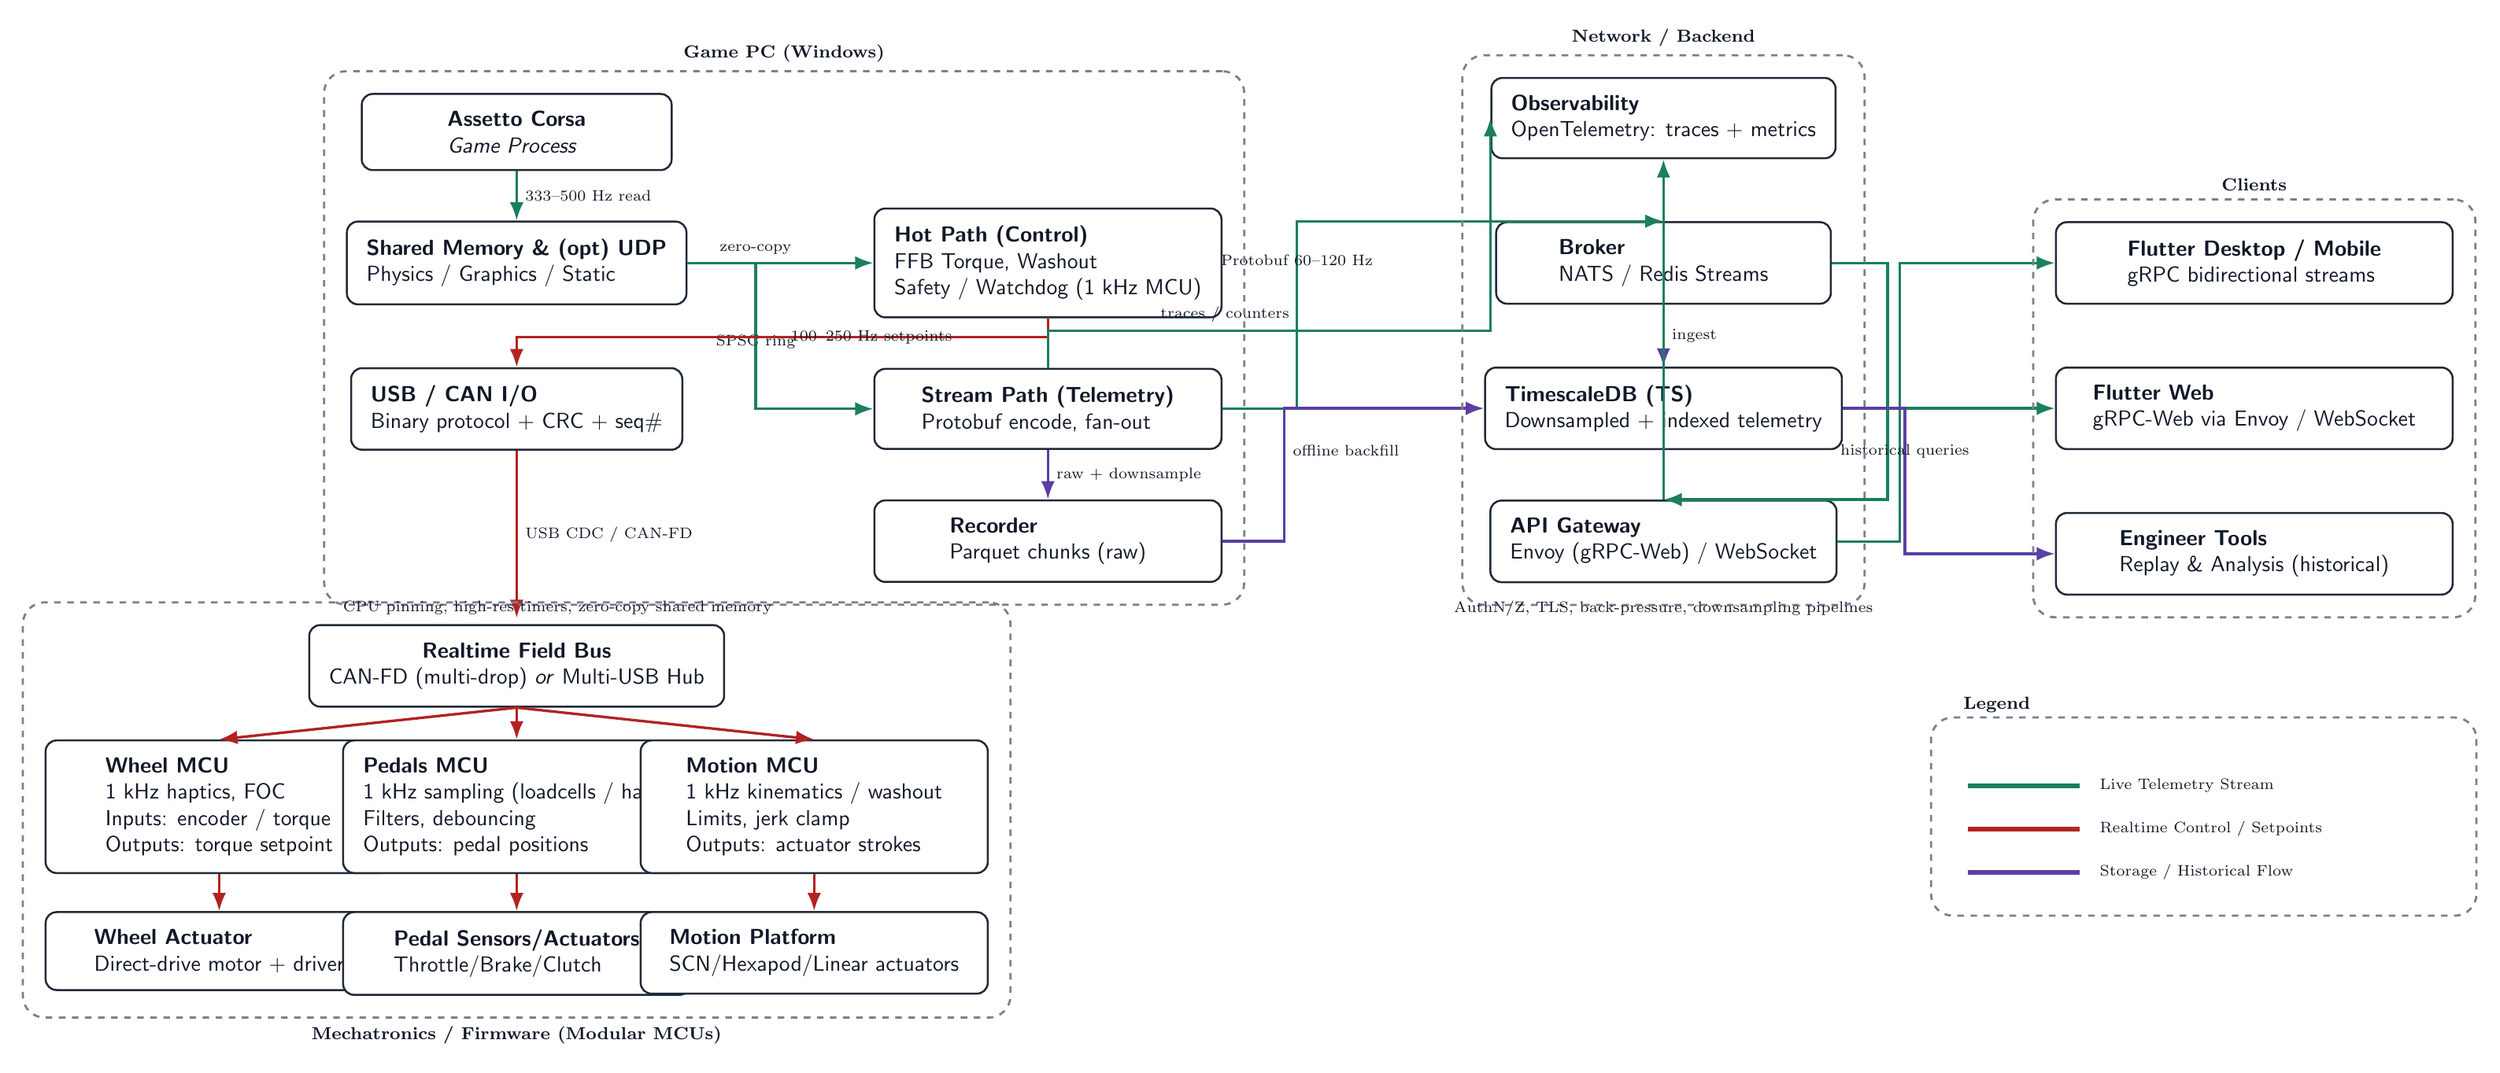
\begin{tikzpicture}

% ================== NODES ==================

% --- Game PC stack ---
\node[box, minimum width=50mm] (game) at (0,0) {\textbf{Assetto Corsa}\\\textit{Game Process}};
\node[box, below=8mm of game, minimum width=50mm] (sharedmem) {\textbf{Shared Memory \& (opt) UDP}\\Physics / Graphics / Static};

\node[box, right=30mm of sharedmem, minimum width=56mm, align=left] (hotpath) {\textbf{Hot Path (Control)}\\FFB Torque, Washout\\Safety / Watchdog (1 kHz MCU)};
\node[box, below=8mm of hotpath, minimum width=56mm, align=left] (streampath) {\textbf{Stream Path (Telemetry)}\\Protobuf encode, fan-out};
\node[box, below=8mm of streampath, minimum width=56mm, align=left] (recorder) {\textbf{Recorder}\\Parquet chunks (raw)};

\node[box, below=10mm of sharedmem, minimum width=50mm] (io) {\textbf{USB / CAN I/O}\\Binary protocol + CRC + seq\#};

% --- Distributed Mechatronics (modular MCUs) ---
% field bus / hub directly below IO; pushed far down to avoid Game PC overlap
\node[box, below=28mm of io, minimum width=64mm, align=center] (bus) {\textbf{Realtime Field Bus}\\CAN-FD (multi-drop) \textit{or} Multi-USB Hub};

% three MCU islands
\node[box, minimum width=56mm, align=left] (mcu_wheel) at ($(bus.south)+(-48mm,-16mm)$) {\textbf{Wheel MCU}\\1 kHz haptics, FOC\\Inputs: encoder / torque\\Outputs: torque setpoint};
\node[box, minimum width=56mm, align=left] (mcu_pedals) at ($(bus.south)+(0mm,-16mm)$) {\textbf{Pedals MCU}\\1 kHz sampling (loadcells / halls)\\Filters, debouncing\\Outputs: pedal positions};
\node[box, minimum width=56mm, align=left] (mcu_motion) at ($(bus.south)+(48mm,-16mm)$) {\textbf{Motion MCU}\\1 kHz kinematics / washout\\Limits, jerk clamp\\Outputs: actuator strokes};

\node[box, below=6mm of mcu_wheel, minimum width=56mm, align=left] (act_wheel) {\textbf{Wheel Actuator}\\Direct-drive motor + driver};
\node[box, below=6mm of mcu_pedals, minimum width=56mm, align=left] (act_pedals) {\textbf{Pedal Sensors/Actuators}\\Throttle/Brake/Clutch};
\node[box, below=6mm of mcu_motion, minimum width=56mm, align=left] (act_motion) {\textbf{Motion Platform}\\SCN/Hexapod/Linear actuators};

% --- Network / Backend ---
\node[box, right=44mm of hotpath, minimum width=54mm, align=left] (broker) {\textbf{Broker}\\NATS / Redis Streams};
\node[box, below=10mm of broker, minimum width=54mm] (tsdb) {\textbf{TimescaleDB (TS)}\\Downsampled + indexed telemetry};
\node[box, below=8mm of tsdb, minimum width=54mm, align=left] (gateway) {\textbf{API Gateway}\\Envoy (gRPC-Web) / WebSocket};
\node[box, above=10mm of broker, minimum width=54mm, align=left] (obs) {\textbf{Observability}\\OpenTelemetry: traces + metrics};

% --- Clients ---
\node[box, right=36mm of broker, minimum width=64mm, align=left] (flutterDesktop) {\textbf{Flutter Desktop / Mobile}\\gRPC bidirectional streams};
\node[box, below=10mm of flutterDesktop, minimum width=64mm, align=left] (flutterWeb) {\textbf{Flutter Web}\\gRPC-Web via Envoy / WebSocket};
\node[box, below=10mm of flutterWeb, minimum width=64mm, align=left] (tools) {\textbf{Engineer Tools}\\Replay \& Analysis (historical)};

% ================== FLOWS ==================
\draw[telem] (game.south) -- node[right, small]{333–500 Hz read} (sharedmem.north);

\draw[telem] (sharedmem.east) -- ++(11mm,0) |- node[pos=0.22, above, small]{zero-copy} (hotpath.west);
\draw[telem] (sharedmem.east) -- ++(11mm,0) |- node[pos=0.22, below, small]{SPSC ring} (streampath.west);

\draw[storage] (streampath.south) -- node[right, small]{raw + downsample} (recorder.north);
\draw[control] (hotpath.south) -- ++(0,-3mm) -| node[pos=0.25, right, small]{100–250 Hz setpoints} (io.north);

% IO down to bus
\draw[control] (io.south) -- node[right, small]{USB CDC / CAN-FD} ($(bus.north)+(0,1mm)$);

% bus fanout to MCUs
\draw[control] (bus.south) -- (mcu_wheel.north);
\draw[control] (bus.south) -- (mcu_pedals.north);
\draw[control] (bus.south) -- (mcu_motion.north);

% MCUs to actuators/sensors
\draw[control] (mcu_wheel.south) -- (act_wheel.north);
\draw[control] (mcu_pedals.south) -- (act_pedals.north);
\draw[control] (mcu_motion.south) -- (act_motion.north);

% telemetry/control to backend/clients
\draw[telem] (streampath.east) -- ++(12mm,0) |- node[pos=0.36, above, small]{Protobuf 60–120 Hz} (broker.north);
\draw[storage] (broker.south) -- node[right, small]{ingest} (tsdb.north);
\draw[storage] (recorder.east) -- ++(10mm,0) |- node[pos=0.34, right, small]{offline backfill} (tsdb.west);
\draw[telem] (broker.east) -- ++(9mm,0) |- (gateway.north);

\draw[telem] (gateway.east) -- ++(10mm,0) |- (flutterDesktop.west);
\draw[telem] (gateway.east) -- ++(10mm,0) |- (flutterWeb.west);
\draw[storage] (tsdb.east) -- ++(10mm,0) |- node[pos=0.2, above, small]{historical queries} (tools.west);

\draw[telem] (streampath.north) -- ++(0,6mm) -| node[pos=0.2, above, small]{traces / counters} (obs.west);
\draw[telem] (gateway.north) -- ++(0,6mm) -| (obs.south);

% ================== BOUNDARIES ==================
\node[boundary, fit={(game) (sharedmem) (hotpath) (streampath) (recorder) (io)} , label={[title]above:Game PC (Windows)}] (pcbox) {};
\node[boundary, fit={(bus) (mcu_wheel) (mcu_pedals) (mcu_motion) (act_wheel) (act_pedals) (act_motion)} , label={[title]below:Mechatronics / Firmware (Modular MCUs)}] (fwbox) {};
\node[boundary, fit={(broker) (tsdb) (gateway) (obs)} , label={[title]above:Network / Backend}] (netbox) {};
\node[boundary, fit={(flutterDesktop) (flutterWeb) (tools)} , label={[title]above:Clients}] (clientsbox) {};

% ================== LEGEND (bottom-right) ==================
\coordinate (L0) at ($(clientsbox.south east)+(0mm,-16mm)$);
\draw[boundary, minimum width=88mm, minimum height=32mm] ($(L0)+(0,0)$) rectangle ++(-88mm,-32mm);
\node[title, anchor=west] at ($(L0)+(-84mm,2mm)$) {Legend};
\draw[legendline, draw=clr-telemetry] ($(L0)+(-82mm,-11mm)$) -- ++(18mm,0);
\node[labelbox, anchor=west] at ($(L0)+(-62mm,-11mm)$) {Live Telemetry Stream};
\draw[legendline, draw=clr-control] ($(L0)+(-82mm,-18mm)$) -- ++(18mm,0);
\node[labelbox, anchor=west] at ($(L0)+(-62mm,-18mm)$) {Realtime Control / Setpoints};
\draw[legendline, draw=clr-storage] ($(L0)+(-82mm,-25mm)$) -- ++(18mm,0);
\node[labelbox, anchor=west] at ($(L0)+(-62mm,-25mm)$) {Storage / Historical Flow};

% ================== NOTES ==================
\node[small, anchor=north west] at ($(pcbox.south west)+(2mm,2mm)$) {CPU pinning, high-res timers, zero-copy shared memory};
\node[small, anchor=north] at ($(netbox.south)+(0,2mm)$) {AuthN/Z, TLS, back-pressure, downsampling pipelines};

\end{tikzpicture}
\end{document}
